\chapter{Wykład 5. Zarządzanie projektami wg metodyki PMBOK}

\section{Analiza wartości}
% strona 14
\subsection*{Dokonaj analizy wartości PMBOK, które mogą być przydatne w projekcie.}

Wartości, które mogą być przydatne w projekcie:
\begin{itemize}
\item profesjonalizm działania i etyka zawodowa, 
\item kompetentna kadra zarządzająca projektem ,
\item profesjonalne zachowanie w trakcie realizacji projektu,
\item ogólny i globalny charakter metodyki,
\item skalowanie metodyki, 
\item dostarczenie klientowi projektu dokładnie takiego jakiego wymagał,
\item wartościowanie wymagań,
\item plan i pro aktywne działanie,
\item planowanie kroczące i poprawa planów,
\item zintegrowane zarządzanie zmianą. 
\end{itemize}

\subsection*{Wyznacz zasady i wartości dla Twojego projektu.}

Zasady i wartości dla naszego projektu:
\begin{itemize}
\item ustalone reguły zachowania i postępowania,
\item konsekwentne postępowanie według przyjętego plany,
\item omawianie potencjalnych konfliktów,
\item wspólne rozwiązywanie problemów,
\item trzymanie się ustalonego sposobu raportowania, jak najszybsze informowanie o zmianach,
\item spotkania, które pozwolą na przedstawienie różnych punktów widzenia.
\end{itemize}

% ===========================================================================

\section{Role i struktury organizacyjne}
% strona 51

Role w PMBOK:
\begin{enumerate}
\item	Wykonawca projektu (Project Performer) – osoba/organizacja odpowiedzialna za projekt.
	\begin{enumerate}
	\item	Zespół projektowy (Project Team) – zespół składający się zarówno z osób zajmujących się zarządzaniem projektem jak i  osób wykonujących pracę nad produktem wyjściowym.  Zespół projektowy wykonując swoje obowiązki dąży do dostarczenia produktu.
		\begin{enumerate}
		\item	Zespół rozwijający project (Project Development Team) – zespół odpowiedzialny za wykonywanie pracy związanej z wytworzeniem produktu i spełnieniem narzuconych wymagań.
		\item	Zespół zarządzania projektem (Project Management Team) – zespół odpowiedzialny za planowanie, kontrolowanie i monitorowanie pracy nad projektem. Zespół wspiera Kierownika projektu dostarczając mu niezbędnych informacji uzyskanych podczas procesu monitorowania projektu.
		\end{enumerate}
	\item	Kierownik projektu (Project Manager) – jest odpowiedzialny za planowanie i organizację pracy podczas realizacji projektu. Zarządza wszystkimi działaniami codziennymi. PM odpowiada za dostarczenie klientowi produktu. Jest to osoba reprezentująca projekt na zewnątrz oraz odpowiadająca za jego sukces.
	\item	Kierownik funkcjonalny (Functional Manager) – jest odpowiedzialny za zarządzanie szeroko pojętym biznesem, czyli finansami, kontraktami oraz zasobami ludzkimi.
	\item	Rada kontroli zmian (Change Control Board) – grupa zajmująca się kontrolowaniem zmian w projekcie. Grupa ma prawo zarówno do akceptacji jak i odrzucenia zmian w projekcie. 
	\item	Biuro zarządzania projektem (PMO – Project Management Office) – jednostka wspierająca zarządzaniem projektem w przedsiębiorstwie. Biuro projektowe wspiera projekt pod kątem administracyjnym – zarządza dokumentacją, zasobami ludzkimi i przebiegiem projektu.
	\end{enumerate}
\item	Klient (Customer) – kupujący produkt lub usługę wytworzone podczas projektu.  
\item	Użytkownik (User) – rodzaj klienta nie będącego bezpośrednim nabywcą produktu. Użytkownik korzysta  z produktu.
\item	Inwestor (Sponsor) – osoba (lub grupa osób) dostarczająca środków finansowych na realizację projektu, mająca znaczny wpływ na zakres projektu. Inwestor jest osobą odpowiedzialną za akceptację produktu.

Zleceniodawca (Project Customer) – typ inwestora zlecającego wykonanie projektu w formie kontraktu. 
\item	Sprzedawca (Seller) – osoba/organizacja/przedsiębiorstwo sprzedająca/e produkt lub usługę. Sprzedawca nie musi być wytwórcą produktu.
\end{enumerate}

W PMBOK nie ma jasno określonej definicji struktury organizacyjnej. Struktury organizacyjne tworzy się w celu realizacji wyspecyfikowanych zadań. Można wyróżnić kilka typów struktur organizacyjnych:
\begin{itemize}
\item	Projektowa – podział per projekt. Kierownik projektu ma silną władzę. 
\item	Funkcjonalna – podział per funkcja. Działy funkcjonalne kierowane przez specjalistów, pracownik podlega więcej niż jednemu kierownikowi.
\item	Macierzowa (Matrix) – połączenie struktury projektowej i funkcjonalnej.
\end{itemize}


\textbf{Wyznacz role i struktury organizacyjne dla Twojego projektu:}


W naszym projekcie występują następujące role:
\begin{itemize}
\item Kierownik Projektu
\item Zespół projektowy
\item Rada kontroli zmian
\item Inwestor
\item Użytkownik
\end{itemize}


Przyjmujemy projektową strukturę organizacyjną:
\begin{figure}[!ht]
\begin{center}
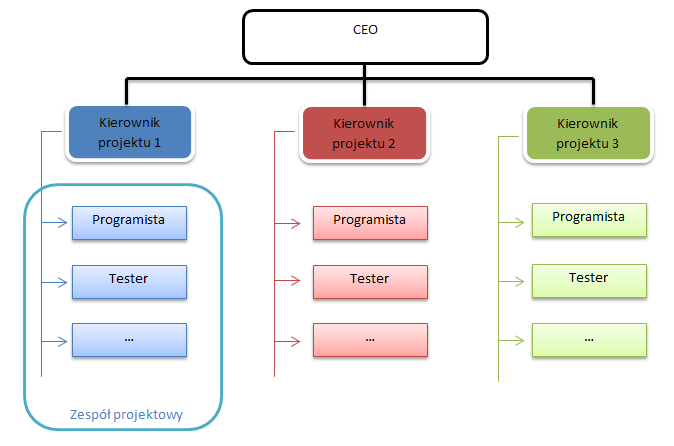
\includegraphics[width=\textwidth]{struktura_org.png}
\caption[Struktura organizacyjna]{Struktura organizacyjna}
\label{rysunekProces}
\end{center}
\end{figure}




